\documentclass[11pt]{elegantbook}
\definecolor{structurecolor}{RGB}{40,58,129}
\linespread{1.6}
\setlength{\footskip}{20pt}
\setlength{\parindent}{0pt}
\newcommand{\argmax}{\operatornamewithlimits{argmax}}
\newcommand{\argmin}{\operatornamewithlimits{argmin}}
\elegantnewtheorem{proof}{Proof}{}{Proof}
\elegantnewtheorem{claim}{Claim}{prostyle}{Claim}
\DeclareMathOperator{\col}{col}
\title{\textbf{STAT 426}}
\author{Wenxiao Yang}
\institute{Department of Mathematics, University of Illinois at Urbana-Champaign}
\date{}
\setcounter{tocdepth}{2}
\cover{cover.jpg}
\extrainfo{All models are wrong, but some are useful.}

% modify the color in the middle of titlepage
\definecolor{customcolor}{RGB}{32,178,170}
\colorlet{coverlinecolor}{customcolor}
\usepackage{cprotect}

\addbibresource[location=local]{reference.bib} % bib

\begin{document}

\maketitle
\frontmatter
\tableofcontents
\mainmatter

\section{Basic of Categorical Data}
\subsection{Variable Measurement}
\begin{center}\begin{figure}[htbp]
    \centering
    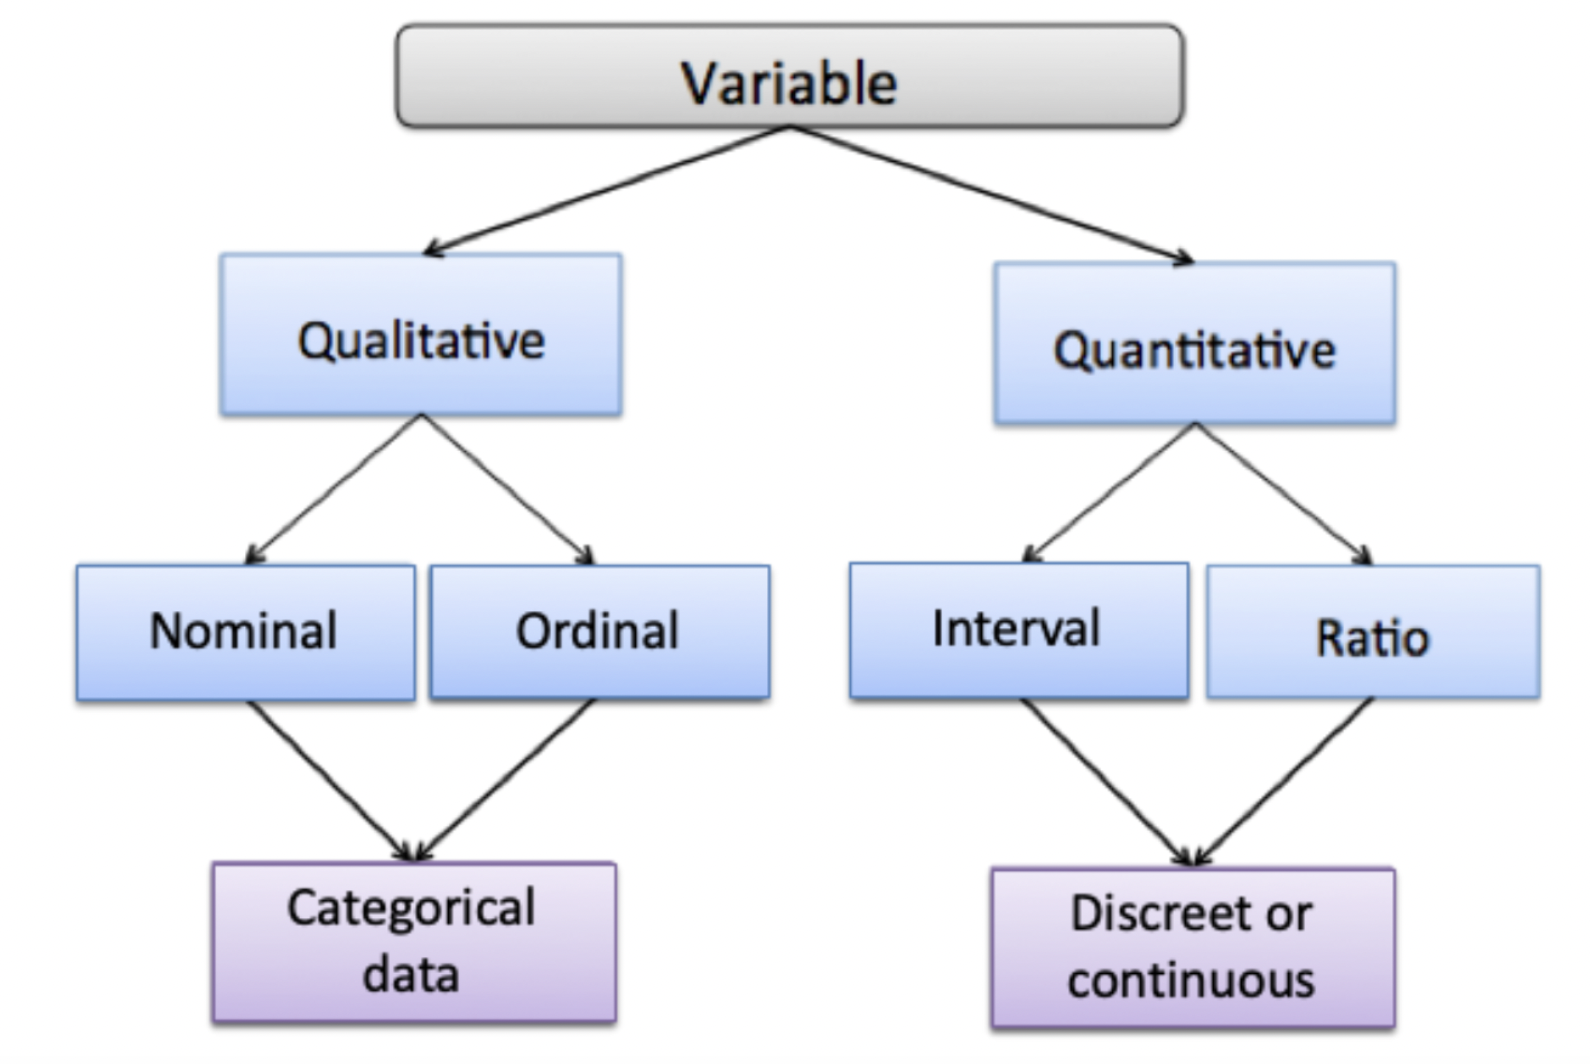
\includegraphics[scale=0.3]{p1.png}
    \caption{Variable Type}
    \label{}
\end{figure}\end{center}
\begin{enumerate}[a)]
    \item Nominal: Categories do not have a natural order. Ex. blood type, gender.
    \item Ordinal: Categories have a natural order. Ex. low/middle/high education level
    \item Interval: There is a numerical distance (difference between two different values is meaningful) between any two values.
    Ex. blood pressure level, 100 blood pressure doesn't mean the double degree of 50 pressure.
    \item Ratio: An interval variable where ratios are valid (presence of absolute zero, i.e. zero is meaningful). Ex. weight, 4g is double degree of 2g.
\end{enumerate}

A variable’s level of measurement determines the statistical methods to be used for its analysis.

Variables hierarchy: Ratio > Interval > Ordinal > Nominal

Statistical methods applied to variables at a lower level can be used with variables at a higher level, but the contrary is not true.























\end{document}